\documentclass{article}
\usepackage[top=2cm, bottom=2cm, left=2cm, right=2cm]{geometry}
\usepackage[english]{babel}
\usepackage{titling}
\usepackage{graphicx}
\usepackage[usenames,dvipsnames]{xcolor}
\usepackage{scrextend}
\changefontsizes[20pt]{12pt}
\usepackage{floatrow}
\usepackage{courier}
\usepackage{caption}
\usepackage{fontspec}
\setmonofont{DejaVu Sans Mono}
\title{Paper 2014 - A talk about Network}
\author{Daniel Maxime (Group 2326)}
\date{August 2014}

\begin{document}
\maketitle
\newpage

\tableofcontents
\clearpage

%
% Like most people we, English lecturers, use computer networks every day.
% We have a vague understanding of what IP addresses are, but what do they refer to exactly?
% There has been a lof a talk about IPv4, IPv6 and even IPv8 more recently.
% What are they? What are the differences?
% 
% Why do we need to mention « ports » in addition to « addresses » ?
% What’s the link between such « ports » and the notion of « service » ?
% Could you give some common examples ?
% 
% Last time we inadvertently opened a network configuration window,
% we came across the word "subnet mask": what is is, and what is it used for?
% 
% Is the subnet mask anything to do with routers?
% Isn't a router a computer ? Or is it the same as a switch?
%


\section{Introduction}
	\subsection{Computers network}
	
	Computers that we all know are useful for a lot of things: managing works, computing for science research,
	making movies, graphics, playing games, ... But computers are more useful when then can communicate with each other !
	On top of all that, they can connect their users between them. That's probably the most important part of a
	computer nowadays. Interacting with computers is useful but using it remotly or contacting a service that
	is on the other side of the Earth, that's just beautiful.
	
	The computer networks have undergone major changes over time. Multiple projects came out and
	only some of them (a single one in fact) survived. Let's see how it works...
	
	\subsection{A brief history}
	
	At first, to communicate with a computer system, you need a common way to "talk" with the others. To achieve
	this, some projects were made to try to unify the system with performance and well minded.
	
	The communication schema and definition (most of the time, this is public and freely accessible under what we
	call RFC (Request For Comments)) used on computer science are called "Protocols".
	Some of them were made to connect computers between them: ARCnet, Ethernet, Token Ring, IP, ...
	
	These protocols were made for the same purpose (connect physically and logically devices) but with different
	working methods. The main difference is the way "how and when devices can talk".
	ARCnet and Token Ring use "tokens" to allow someone to talk or not, Ethernet (which is the most used now)
	talks when he wants and manages collisions (when two people talk at the same time).
	
	I'll only keep protocols which are still used nowadays, everywhere, and skip the others.
	But, how these protocols work together ?

\section{Network layers}

	The mot important part of the network base is the "OSI model" (Open Systems Interconnection model) which characterizes and
	standardizes the internal functions of a communication system. All "Internet" networks use it. This model splits
	the work in 7 layers, each independant from one another. You can changer a layer without affecting the content
	of the others. It's due to this method that you can browse the web on wireless or wired connection without changing
	all your hardware.
	
	Let me explain these layers from the bottom to the top, to understand how each small protocol used on the Internet
	works with the others to provide a full and flexible support. After that, we will see how these protocols interact
	with each other.
	
	\subsection{Layer 1 - Physical layer}
	
	This layer is definitely the easiest layer of the OSI model, it's globally just the wire which connects one
	device to another (your computer to your Internet Provider's box, the Internet Provider's box to their
	data center, etc). In your house, except the "ethernet-cable" or the wireless access, you probably don't have
	any other layer 1 technology, but there are many others.
	
	Now, we have a cable between two devices, that's fine, but how can we make them communicate ?
	With the layer 2 of course.

	\subsection{Layer 2 - Data link layer}
	
	This (single) layer enables devices to communicate together on a small area (eg: devices you have at your house,
	nothing more). The most common protocol used at this layer is Ethernet. This protocol is made to transmit data
	over the layer 1, with some collisions and errors detection. After that, to connect two devices between them, you
	need to use addresses. Ethernet use MAC addresses.
	\footnote{No, you don't need to have an "Apple Mac Computer" to have a MAC address.
	All physical ethernet network cards have got a unique one on the world.}
	\footnote{Exemple of MAC address: 00:54:77:65:78:21}
	A MAC address is 48 bits longs, that means that there are about 281,000 billion addresses possible. I think that's
	enough for your home (yes, remember, this protocol connects only a small area).
	
	This protocol, like all protocols (you will see later) uses a generic data representation:
	header + payload (+ footer).
	The footer is not always present on every protocol, but often, this is where the "checksum" (a small amount of data
	which enables corruption detection) is put.
	
	The header is dedicated for Ethernet, the payload is simply used to put
	the layer 3 on it. This method is called "encapsulation" (like Matriochka dolls), it's with this method that all layers
	will be put together.
	
	To communicate with someone, we must know their address, but when we talk to someone, it's a good idea to
	get their response. To help them respond, we will provide our address too. Well, the header will contain
	at least the destination address and the source address (ours). This will be the same for all the protocols
	that we'll see.
	
	Now we can connect two devices and exchange data (on the payload) between them. Let's see how we can extend
	the area of communication (Internet in your home only is not very interesting).
	
	\subsection{Layer 3 - Network layer}
	
	To extend your connectivity all around the world, using MAC addresses only is not possible due to conception
	of the protocol: Ethernet, as I said is made for local traffic. To extends this traffic to the outside, we need
	to use another protocol, which is made for that. It's called IP (Internet Protocol). Yes, this is the protocol
	which is really used to have "Internet".
	
	Nice, but, what exactly is IP ? IP is the protocol which enables to make the link with the underlying layer
	and global mapped address. IP uses... IP addresses.
	\footnote{Exemple of IP address: 82.212.175.9} to represents source and destination. With the fourth version of the protocol
	(commonly called IPv4), addresses are 32 bits long, which makes about 4 billions unique addresses. At the beginning of
	the "Internet time", this was absolutely huge.
	
	One more time, we will encapsulate this protocol on the underlying protocol. We have this schema right now:
	\begin{center}
	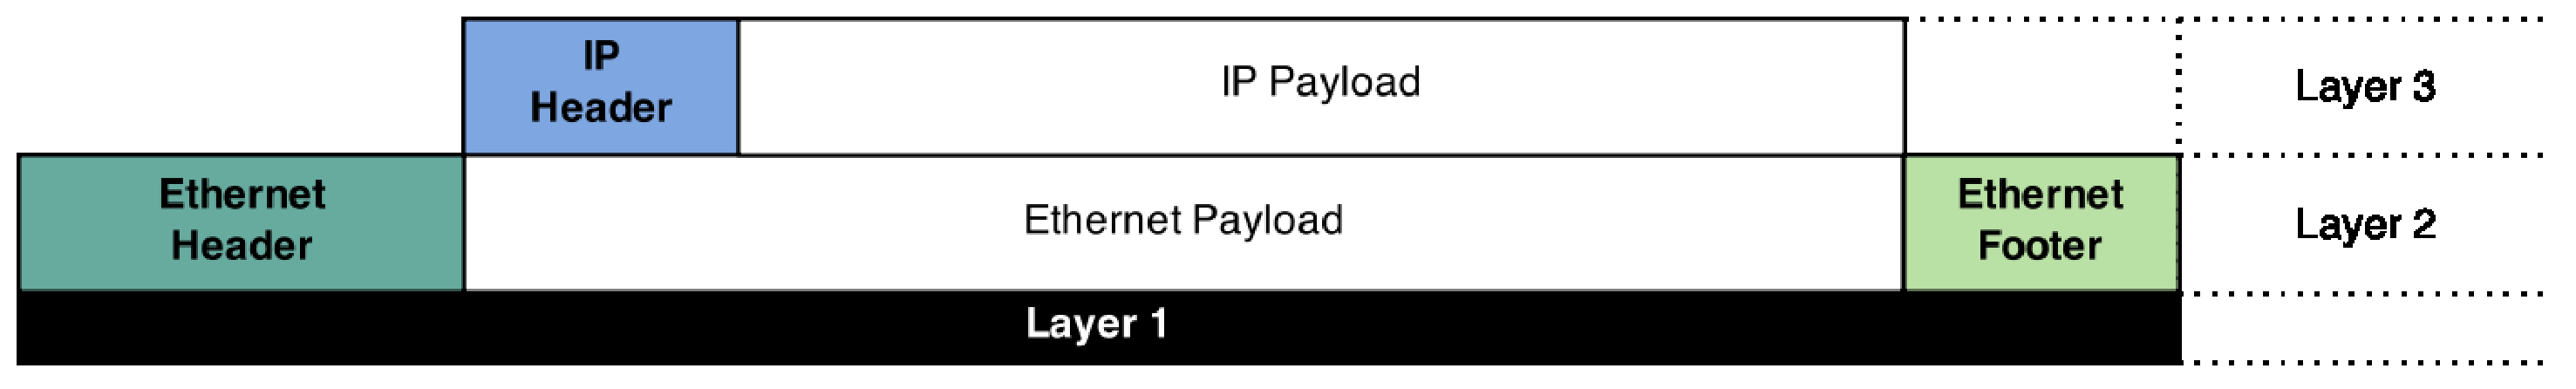
\includegraphics[scale=0.3]{content/layer3.eps}
	\end{center}
	
	We can now contact devices outside our home. We will see later how and why it's only now that we can contact
	the "outside world". That's nice, but how can I contact a specific service (web browser, file transfert, chat, ...)
	on a specific device, we only know its address right now.
	
	\subsection{Layer 4 - Transport layer}
	
	To understand a little bit more how that works, I'll draw an analogy with real life. Imagine a world with
	roads and a lot of buildings with flats. Roads are the layer 1 (wire), your car is the layer 2 (Ethernet), the building
	address, flat stage and flat number are described by the IP address. Now you are at your destination, you want to
	go to a specific location on this flat. When your enter the flat, you are in the lobby, you have multiple doors
	in front of you. That's the solution. Behind each doors you have one service.
	
	These doors on network are called "ports".
	
	This happen on layer 4 with multiple possible protocols. The most used are TCP and UDP. They are both the same purpose
	and differents ports, but work in two different ways, these ways are not important to understand how it works.
	ss
	Just keep in mind that these ports enable you to access specific services on the remote device. Like each time,
	this works with encapsulation. That's what we have after this encapsulation:
	\begin{center}
	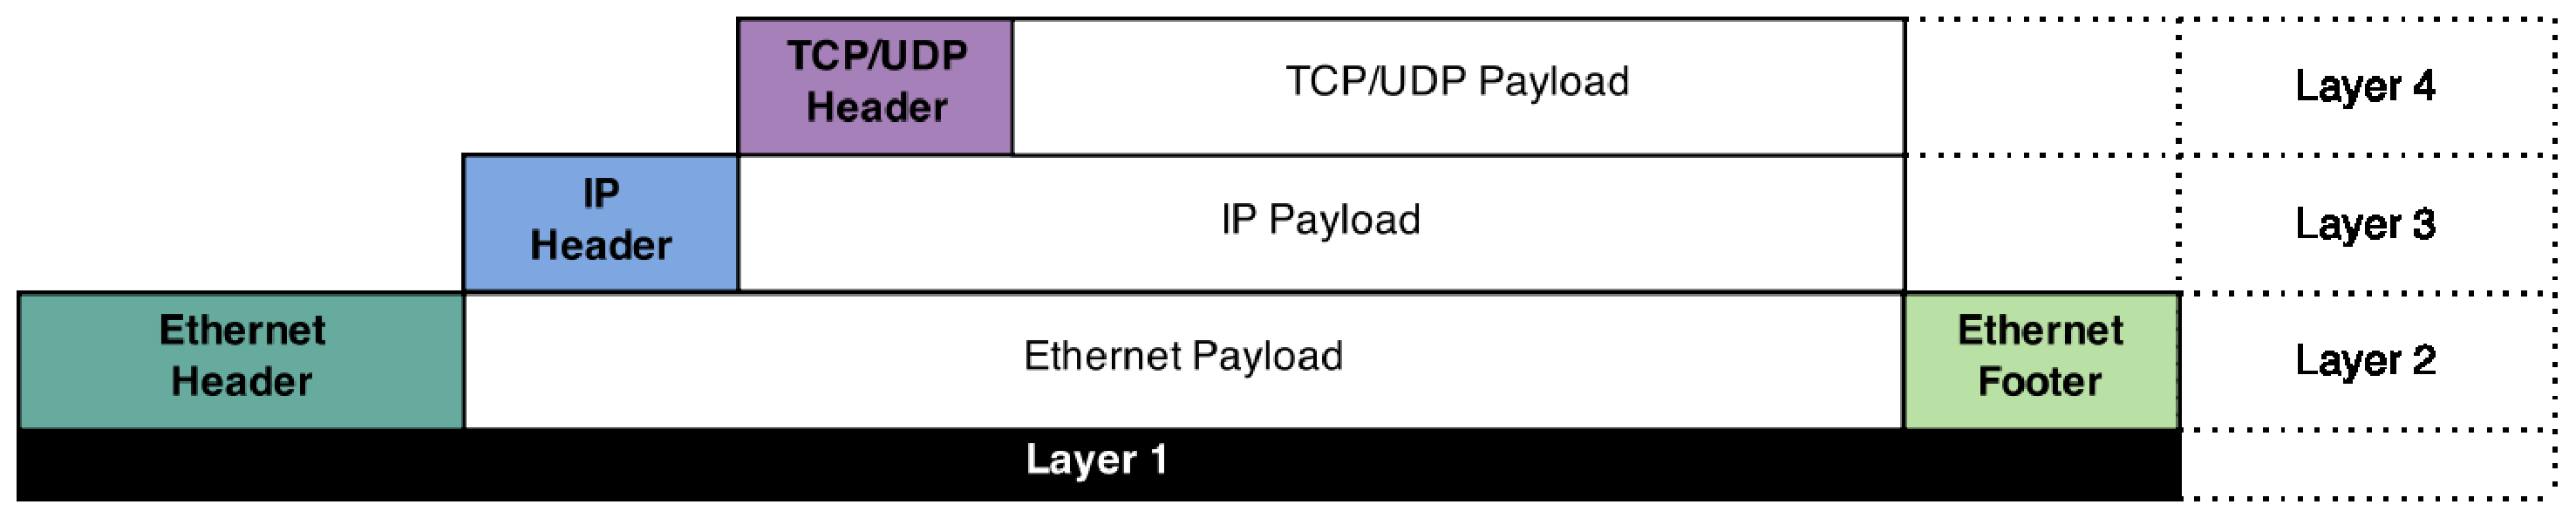
\includegraphics[scale=0.3]{content/layer4.eps}
	\end{center}
	
	Like before, the header contains the source port and the destination port. Yes, you have a source port. In fact,
	a webserver is a service behind a door and your web browser is a service too, but behind a door at your home.
	That explains how you can browse multiple and different websites at the same time: everything has its own door (port).
	
	And voila. You can communicate and exchange data with your correspondant ! But what kind of data ?
	
	\subsection{Layer 7 - Application layer}
	
	We are now at layer 7. What ? And what about layer 5 and 6 ? They are not important for us, we can skip them, most
	of the time, these layers are not used at all because we don't need them.
	
	Well, what is the layer 7 ? It's simply data you want to exchange. You can send "hello" (really just "hello"),
	and that's what the remote service (remember, the door) will receive. That's easy but to request a web page for example,
	we must provide a comprehensive way to talk with the web server. To perform that correctly, we use... one more time,
	protocols ! At this layer, we find a lot of protocols: http, ftp, ssh, irc, telnet, smtp, pop3, imap, ...
	
	Each of these protocols has a default port number. The exact content of the protocol is described on each RFC
	specially written for that.
	
	Now, our complete frame looks like that:
	\begin{center}
	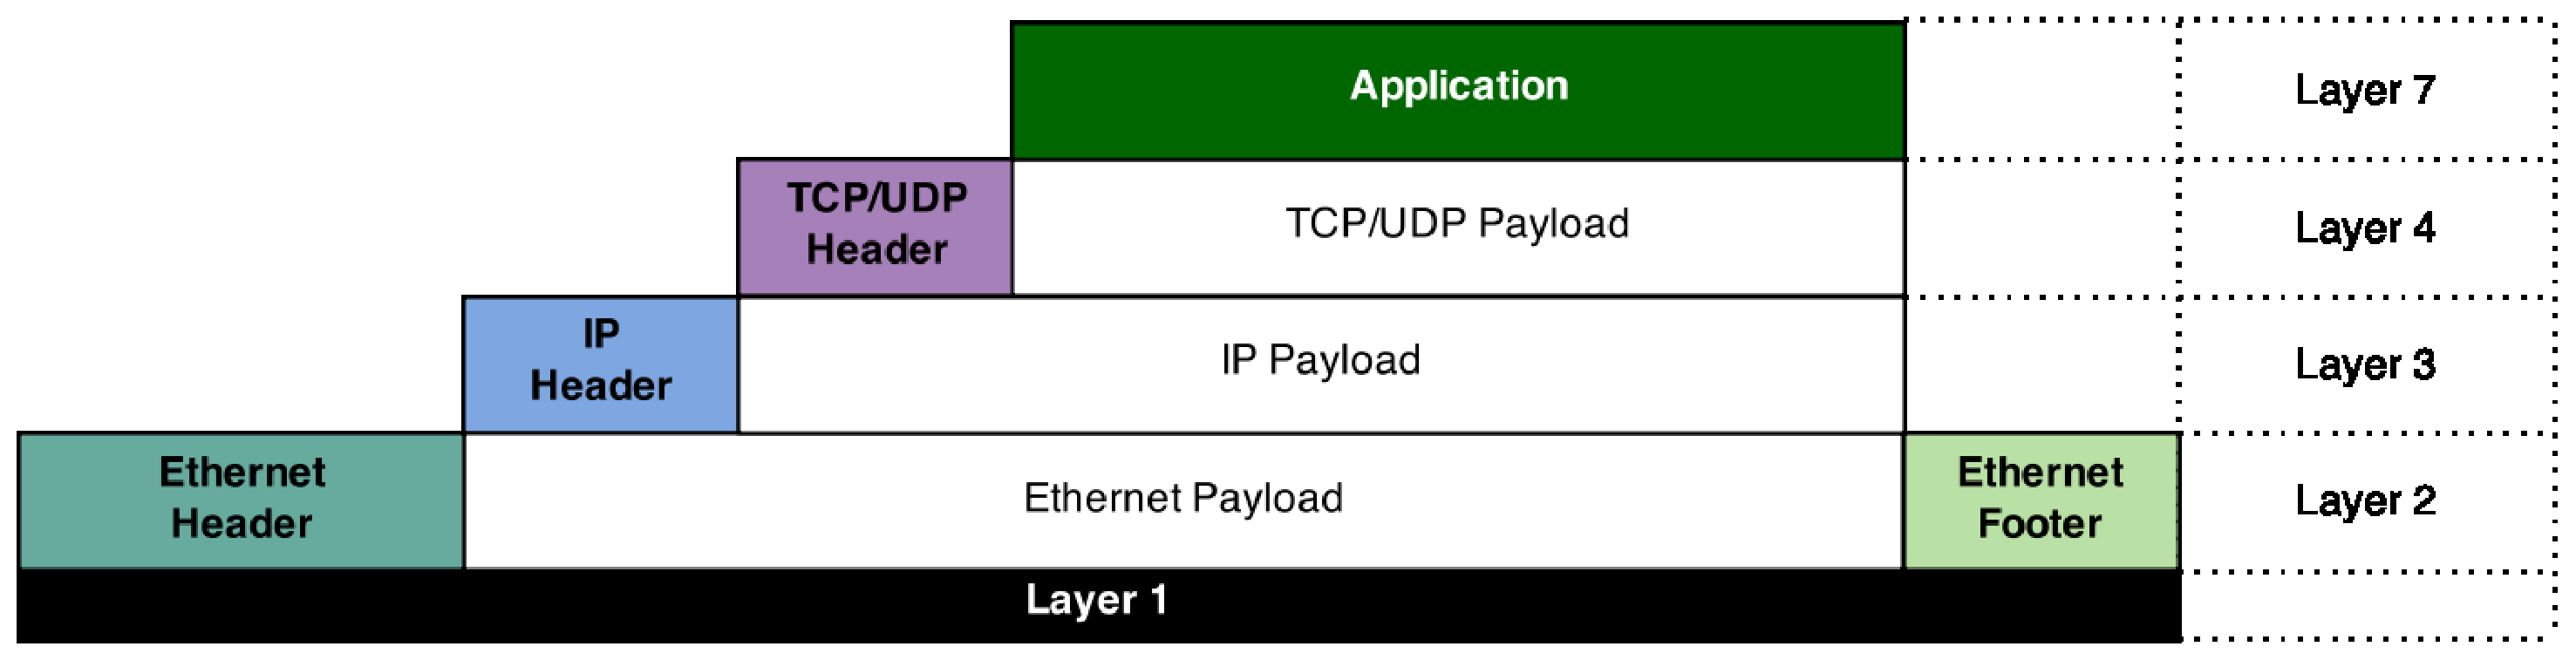
\includegraphics[scale=0.3]{content/layer7.eps}
	\end{center}
	
	That's nice, but why do we need all of these protocols to reach the wanted destination, and why do we split them?
	To understand that, we must go deeper in the description.

\section{A little deeper...}
	You have (I hope) the schema with building, flats and roads on your mind. Keep it fresh, I'll complete it to 
	understand well some devices and specific additionnal services you can find on networks.
	
	For specific reasons, flats can communicate with layer 2 at the same floor only (you have probably 3 or 4 flats
	per stages). To communicate between flats, we need to connect them to each other. For that we will use a "switch".
	This device's job is just to send traffic (based on the destination MAC address) on the right wire connected.
	
	To communicate with your building (without going outside your building I mean), you need to connect each stages between
	them. You can use a switch to connect the stages between them (that's pretty easy right ?). Each flat has its own
	IP address, and to segments all the Internet IP Addresses, we will split them per building. Each building has its own
	part of "The Internet (IP)". This part is called "subnet". With this feature, you can communicate with your building
	without additionnal devices or something else. You are isolated.
	
	To make buildings communicate with others, you need to put a device on the building door, which will work on the
	link between the building and the road. To access some roads and know which road to take, we use a device
	which knows these road... or more precisely, these routes ! This device is called... a router. Easy right ?
	
	The job of a router is just to connect your sub-network with others.
	
	Another interesting thing that we can put on the building is a security agent. We can put one on the router to
	control who enters and goes out the building, and we can put a security agent on each flat, to control who comes in, 
	trying to access some services. If this security agent sees someone unauthorized, he will simply throw them out.
	This security agent is called "firewall".
	
	That's all folks ! You now know basically how a computer network works. Pretty simple, right ? That's how it works
	nowadays, but computer science is a science which progresses everyday and the futur is already considered.

\section{What's next ?}
	Remember, I explained to you the layer 3 with the fourth version of "IP" (IPv4). Nowadays, IPv6 exists. In fact, the
	IPv4's 32 bits long addresses are too short now. We'll reach the limit of existing addresses very soon, that's the
	main reason for IPv6 to exists. The main new thing that IPv6 improves is that the addresses are no more on 32 bits,
	but on 128 bits. That puts the limit at approximately 3.4x$10^{38}$ addresses. This is really really big.
	This is not the only one change with IPv6, some technical details change too. IPv4 is more than 30 years old, 
	since then, we found and improved IPv6 with some missing or some deprecated features.
	
	To enable everyone to have IPv6 at their home, the world must use a software IPv6-capable. But the avantage of a
	layered system is that we only need to change the layer 3 in the whole system, the other layers remain unchanged. That means
	that HTTP, TCP and Ethernet still work the same way on IPv4 or IPv6. That's so beautiful !
	
	Finally, if you've heard of IPv8, IPv9 or something like that, forget it, they simply don't exist.
	\newpage

\section{Conclusion}
	You now know how computers networks (Internet mainly) works, with which protocols and how they communicate with each other.
	Your network card contains a MAC address used by IP to go outside your house. You have ports which specify the service
	and the application protocol which contains your requests for specific services.
	
	\newpage

\section{Sources}
	\begin{itemize}
		\itemsep0em
		\item https://en.wikipedia.org/wiki/Ethernet
		\item https://en.wikipedia.org/wiki/Internet\_Protocol
		\item https://en.wikipedia.org/wiki/MAC\_address
		\item https://en.wikipedia.org/wiki/ARCnet
		\item https://en.wikipedia.org/wiki/TokenRing
		\item https://en.wikipedia.org/wiki/OSI\_model
		\item Graphics are made using https://draw.io
	\end{itemize}
	
\end{document}







